\documentclass[sigplan,11pt,nonacm]{acmart}
\settopmatter{printfolios}

\usepackage{booktabs} % For formal tables
\usepackage{subcaption}
\usepackage{tikz}
\usepackage{pgfplots}
\usepackage{pgfplotstable}
\usepackage{hyphenat}
\usepackage{todonotes}
\usepackage[babel]{csquotes}

\begin{document}
\title[State of LLVM's Vectorization Plan]{Utilizing Parallel Workers: LLVM's Vectorization Plan}
\author{Jonas Fritsch}
\affiliation{%
  \institution{Technical University of Munich}
}
\email{jonas.fritsch@tum.de}

\begin{abstract}
  Modern SIMD processors provide various vector registers and ISAs for programmers to utilize. 
  However, manually vectorizing code can be time-consuming, so compilers look to auto-vectorize 
  code for better performance. LLVM, as a widely used compiler toolchain, could only auto-vectorize 
  basic scalar code. Intel proposed a comprehensive refactoring of the underlying system to enable 
  LLVM's auto-vectorization to support more complex optimizations. The suggested Vectorization Plan 
  (VPlan) architecture would be more modular and scalable. Since then, significant efforts have been 
  made to implement this new system. Today, VPlan is already actively involved in vectorizing 
  innermost loops. Other areas, such as outer loop vectorization, are also in development.
  In this paper we give an introduction into VPlan and summarize its latest development results.
\end{abstract}

\maketitle

%%%%%%%%%%%%%%%%%%%%%%%%%%%%%%%%%%%%%%%%%%%%%%%%%%%%%%%%%%%%%%%%%%%%%%%%%%%%%%%%%%%%%%%%%%%%%%%%%%%%%%
%%%%%%%%%%%%%%%%%%%%%%%%%%%%%%%%%%%%%%%%%%%%%%%%%%%%%%%%%%%%%%%%%%%%%%%%%%%%%%%%%%%%%%%%%%%%%%%%%%%%%%
%%%%%%%%%%%%%%%%%%%%%%%%%%%%%%%%%%%%%%%%%%%%%%%%%%%%%%%%%%%%%%%%%%%%%%%%%%%%%%%%%%%%%%%%%%%%%%%%%%%%%%


\section{Introduction}
\label{sec:introduction}
Modern CPUs are often equipped with multiple different vector registers. These registers are nowadays 
as wide as 512 bits, allowing for the processing of multiple data streams at once (SIMD). By 
batching multiple values together in one register, different ISAs like Intel AVX or ARM SVE allow 
the execution of the same instruction for all values in a vector register simultaneously. 
Utilizing this leads to significant performance improvements over the scalar equivalent most of 
the time.

However, manual code vectorization can quickly become time-consuming, especially when
supporting different CPU architectures. Modern compilers aim to automatically transform scalar code
to use vectorization when applicable.

As one of the most widely used compilation frameworks, LLVM~\cite{10.5555/977395.977673} has 
implemented and refined its auto-vectorization over many years. It provides two different 
Vectorizers, one for innermost loops (LoopVectorize) and one for super-word parallelism 
(SLPVectorize)~\cite{llvmvec}.

This system, however, had quite a few limitations, as the loop vectorizer could only handle
innermost loops and neither outer loops, complex control flow, nor non-inlined functions. 
Additionally, while multiple different vectorizations for the same scalar code 
would be possible, the current vectorizers working directly on the LLVM IR could not model
and compare the costs of such different vectorization approaches.

With these limitations in mind, Intel started an ongoing refactorization effort to migrate LLVM's
auto-vectorization pipeline to utilize a more abstract Vectorization Plan 
(VPlan)~\cite{llvmextloopvec,llvmvplan}. The final goal would be to unite LLVM's auto-vectorization
in a single flexible system capable of optimizing SLPs, inner, and nested loops with complex 
control flow.

The auto-vectorization pass would create multiple different VPlans, based on initial legality 
checks. Each VPlan represents a different vectorization approaches, by modeling the
underlying scalar control flow with its own abstracted vectorized version. Different VPlan-to-VPlan
transformations can then optimize these abstracted control flows based on a cost model.
After that, the best VPlan, and with it the best vectorization approach, is chosen by the cost model.
This VPlan is then executed, by going over its own vectorized control flow representation and
materializing it back into the underlying LLVM IR.

LLVM's VPlan is currently being integrated into the existing Loop Vectorizer and is
already modeling most inner loop vectorizations and transformations~\cite{llvmvplanupdate}. 
Vectorization for outer loops is also in development and can be enabled by setting 
the \texttt{-enable-\allowbreak vplan-\allowbreak native-\allowbreak path} feature 
flag~\cite{llvmouterloop,llvmouterloopstatus}. 
In the future, the plan will be to merge both of these loop vectorization paths into one. 
Merging the existing SLP Vectorizer with VPlan is also planned.

The rest of this paper is organized as follows. We first explain different vectorization
strategies and vectorization constraints in general and describe the original auto-vectorization
approach in LLVM. Section~\ref{sec:vplan} then introduces the new VPlan approach, focusing on
its most important individual components and gives an outlook on future developments. In 
Section~\ref{sec:relatedwork} we highlight related work to LLVM's auto-vectorization. Concluding,
we summarize VPlan, its current state and potential future.

%%%%%%%%%%%%%%%%%%%%%%%%%%%%%%%%%%%%%%%%%%%%%%%%%%%%%%%%%%%%%%%%%%%%%%%%%%%%%%%%%%%%%%%%%%%%%%%%%%%%%%
%%%%%%%%%%%%%%%%%%%%%%%%%%%%%%%%%%%%%%%%%%%%%%%%%%%%%%%%%%%%%%%%%%%%%%%%%%%%%%%%%%%%%%%%%%%%%%%%%%%%%%
%%%%%%%%%%%%%%%%%%%%%%%%%%%%%%%%%%%%%%%%%%%%%%%%%%%%%%%%%%%%%%%%%%%%%%%%%%%%%%%%%%%%%%%%%%%%%%%%%%%%%%


\section{Background}
\label{sec:background}

\subsection{Vectorization Strategies}
\label{back:vec-strat}
In general, vectorization techniques can be separated into different categories:

\paragraph{Inner Loop Vectorization}
Innermost loops are loops whose body's control flow does not contain any more loops.
Vectorization of these loops is more straightforward as the only option to vectorize is over 
the loop's induction variable.

There are various ways to transform the control flow of a loop to accommodate operating on widened
vector registers. Figure~\ref{fig:inner-loop-vec} shows an example of an if-conversion. Some more
examples can also be found in LLVM's Auto-Vectorization Documentation~\cite{llvmvec}.

\begin{figure}
  \centering
  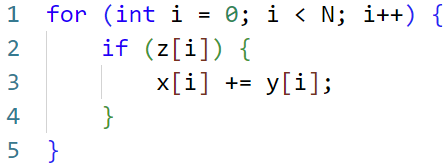
\includegraphics[width=0.35\textwidth]{images/inner-loop-vec.png}
  \caption{A code snippet of a simple loop that would be vectorized over the variable \texttt{i}. 
  The conditional branch would be flattened into a masked addition. The mask would be generated 
  based on \texttt{z[i]}.}
  \label{fig:inner-loop-vec}
\end{figure}

\paragraph{Super-Word Parallelism (SLP) Vectorization}
SLP Vectorization vectorizes similar independent sequential instructions. This can often be seen 
after a loop has been partially or fully unrolled. The resulting similar scalar 
instructions might then be vectorized later by an SLP vectorizer.

\paragraph{Outer Loop Vectorizaton}
Outer loop vectorization focuses on control flow with nested loops. Such control flow often presents
more challenges for auto-vectorization, as one could vectorize over the outer loop,
inner loop, or a mix of both, representing a hybrid/multi-dimensional vectorization approach.
Finding the best legal vectorization can therefor be more difficult.

Figure~\ref{fig:outer-loop-vec} shows a nested loop code snippet where vectorization over the
outer loop would be beneficial.

\begin{figure}
  \centering
  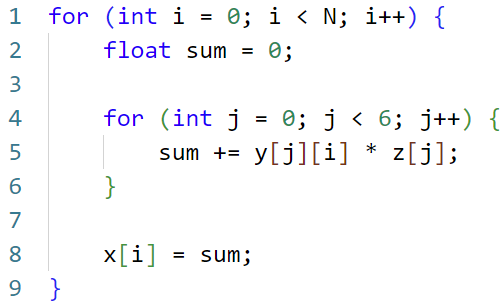
\includegraphics[width=0.39\textwidth]{images/outer-loop-vec.png}
  \caption{A code snippet of a nested loop where it would be beneficial to vectorize over the 
  outer loop. The inner loop has a trip count (6) that is too low to vectorize. Additionally,
  the memory access pattern of \texttt{y} would be consecutive compared to scattered when
  vectorizing over \texttt{i} instead of \texttt{j}.}
  \label{fig:outer-loop-vec}
\end{figure}

\paragraph{Function Vectorization}
Function vectorization refers to the vectorization of entire functions. A loop might contain a
non-inlined function call, passing data related to the iteration variable. During auto-vectorization, 
this call could be replaced with a call to a newly constructed function with the same semantic 
control flow but operating on multiple values at once through vector registers.
 
\subsection{Vectorization Legality}
\label{sec:vec-legal}
Not all loops can be vectorized. There are various factors that can ultimately hinder any
vectorization attempts.

Some of the most common vectorization barriers are data dependencies. As the vectorized version
of a code executes for Vectorization Factor (VF) $N$ data streams simultaneously, it inherently changes
the order of operations. To guarantee that the semantics of the code do not change, all
operations on these $N$ data streams must, generally, be independent. The simplest case
where this is not provided is when the $i$-th loop iteration depends on any of the $(i-N)$-th 
previous iterations.

While explicit data dependencies are easier to see, a simple loop, as in 
Figure~\ref{fig:inner-loop-vec}, could carry an implicit dependency in line 3 if
the \texttt{x} and \texttt{y} point to overlapping memory regions (pointer aliasing).

Not all data dependencies directly hinder any vectorization~\cite{datadepvec}. An exception can, for example, 
sometimes be made for reduction idioms, as seen in the inner loop in 
Figure~\ref{fig:outer-loop-vec}, where \texttt{sum} would be a reduction variable.

Uncountable loops can typically also not be vectorized, due to their unknown number of iterations.

Finally some instructions like integer division do inherently not have a vectorized instruction equivalent.

\subsection{Vectorization Costs}
While vectorizing a given control flow may not be legal, the vectorized code sometimes performs 
worse than its scalar equivalent.

Some control flow transformations that seem beneficial at compile time might reveal a performance
bottleneck at runtime. Considering the code snippet from Figure~\ref{fig:inner-loop-vec}, it might
be that almost all \texttt{z[i]} evaluate to false at runtime. The branch predictor of a CPU
would then be able to guess the correct branch in the scalar code. The vectorized version would
always load the \texttt{y[i]} into memory only for the addition to be masked away. Different 
approaches to avoid such runtime penalties are branch-on-superword-condition code 
(BOSCC)~\cite{10.5555/1299042.1299055,llvmboscc} or active-lane 
consolidation (ALC)~\cite{10.1007/s11227-022-04359-w,10.5555/3615924.3615932}.

Some vector instructions can be costly on most CPUs. Examples are gather, scatter, shuffle,
and permutation instructions. Control flow with many non-adjacent memory loads/stores or 
operations that combine different vector elements, such as reductions, can decrease vectorization 
performance.

Additionally, the vectorized code size will always be larger than the scalar equivalent. This is
due to many factors: (1) The transformed control flow often includes more instructions.
(2) As the loop trip count might not be a perfect multiple of the Vectorization Factor, a scalar
epilogue/remainder of the loop might be used to handle the tail iterations. (3) Various runtime
checks might be inserted throughout the vectorized control flow to handle, for example, pointers 
to overlapping memory regions, in which case the scalar version of the loop is executed.

\subsection{Auto-Vectorization in LLVM}
LLVM implements two different vectorizers for auto-vectorization, LoopVectorize (LV)
and SLPVectorize~\cite{llvmvec,llvmhistorystate}. Auto-Vectorization is part of LLVM's 
middle-end and runs after module simplification has taken place.
In general, these vectorizers take in scalar LLVM IR and transform it into optimized vectorized 
LLVM IR.

SLPVectorize is a SLP vectorizer working on straight-line code (non-loops). It works by analyzing
the code bottom-up, keeping track of dependencies and grouping similar independent scalar instructions
together if possible. Based on a cost model SLPVectorize then decides to vectorize these groups.

LoopVectorize was designed to focus only on vectorization of innermost loops~\cite{llvmintrvplan}. 
When starting with an initial scalable loop in IR, it would first run a legality phase to check 
whether and how it is legal to vectorize the loop. This phase would produce different artifacts, 
such as if 
and what runtime aliasing checks would be required. Then, the cost model ran next, creating more 
cost-based artifacts based on the underlying scalar IR and the legality artifacts. 
Lastly, the transformation phase would vectorize 
the IR in one go based on all the previously produced artifacts.

However, this rigid flow of LoopVectorize presented a challenge. Extending LV to include outer loop 
and nested loop vectorizations would have been difficult, as LV was designed to flatten a
loop's control flow into a single basic block. Producing and considering more and 
more artifacts when trying to transform the scalar loop into a vectorized one all at once also did 
not scale well.

As a potential solution, Intel proposed a long-term effort to refactor LLVM's whole auto-vectorization
using a more modular and flexible system called Vectorization Plan (VPlan)~\cite{llvmextloopvec}.


%%%%%%%%%%%%%%%%%%%%%%%%%%%%%%%%%%%%%%%%%%%%%%%%%%%%%%%%%%%%%%%%%%%%%%%%%%%%%%%%%%%%%%%%%%%%%%%%%%%%%%
%%%%%%%%%%%%%%%%%%%%%%%%%%%%%%%%%%%%%%%%%%%%%%%%%%%%%%%%%%%%%%%%%%%%%%%%%%%%%%%%%%%%%%%%%%%%%%%%%%%%%%
%%%%%%%%%%%%%%%%%%%%%%%%%%%%%%%%%%%%%%%%%%%%%%%%%%%%%%%%%%%%%%%%%%%%%%%%%%%%%%%%%%%%%%%%%%%%%%%%%%%%%%


\section{LLVM's Vectorization Plan}
\label{sec:vplan}

The goal of Intels initial VPlan proposal was to unite any 
auto-vectorization systems (SLP, Inner-/Outer-Loop, Whole-Function) into a single flexible
system~\cite{llvmextloopvec,llvmintrvplan,llvmvplanstate}. 
This system would use VPlans to represent different 
vectorization approaches, abstracting away from the underlying scalar loop IR by using its own 
hierarchical control-flow-graph (H-CFG). This allows for iteratively exploring different 
optimization decisions by performing transformations on this CFG without modifying any LLVM IR.
Each VPlan would be able to calculate its cost and execute itself, materializing the vectorization 
approach back into LLVM IR.

This planned systems is shown in Figure~\ref{fig:vplan-future}. At first, the Legality 
Phase would check if the scalar code would be legal to vectorize at all, and if so, 
initial VPlans would be constructed. In the following Planning Phase, these initial 
VPlans would be optimized using various VPlan-to-VPlan transformations~\cite{llvmouterloopstatus}. 
The VPlan's cost model would supervise those transformations. Finally, the best VPlan 
would be chosen and executed, modifying the underlying IR.

\begin{figure}
  \centering
  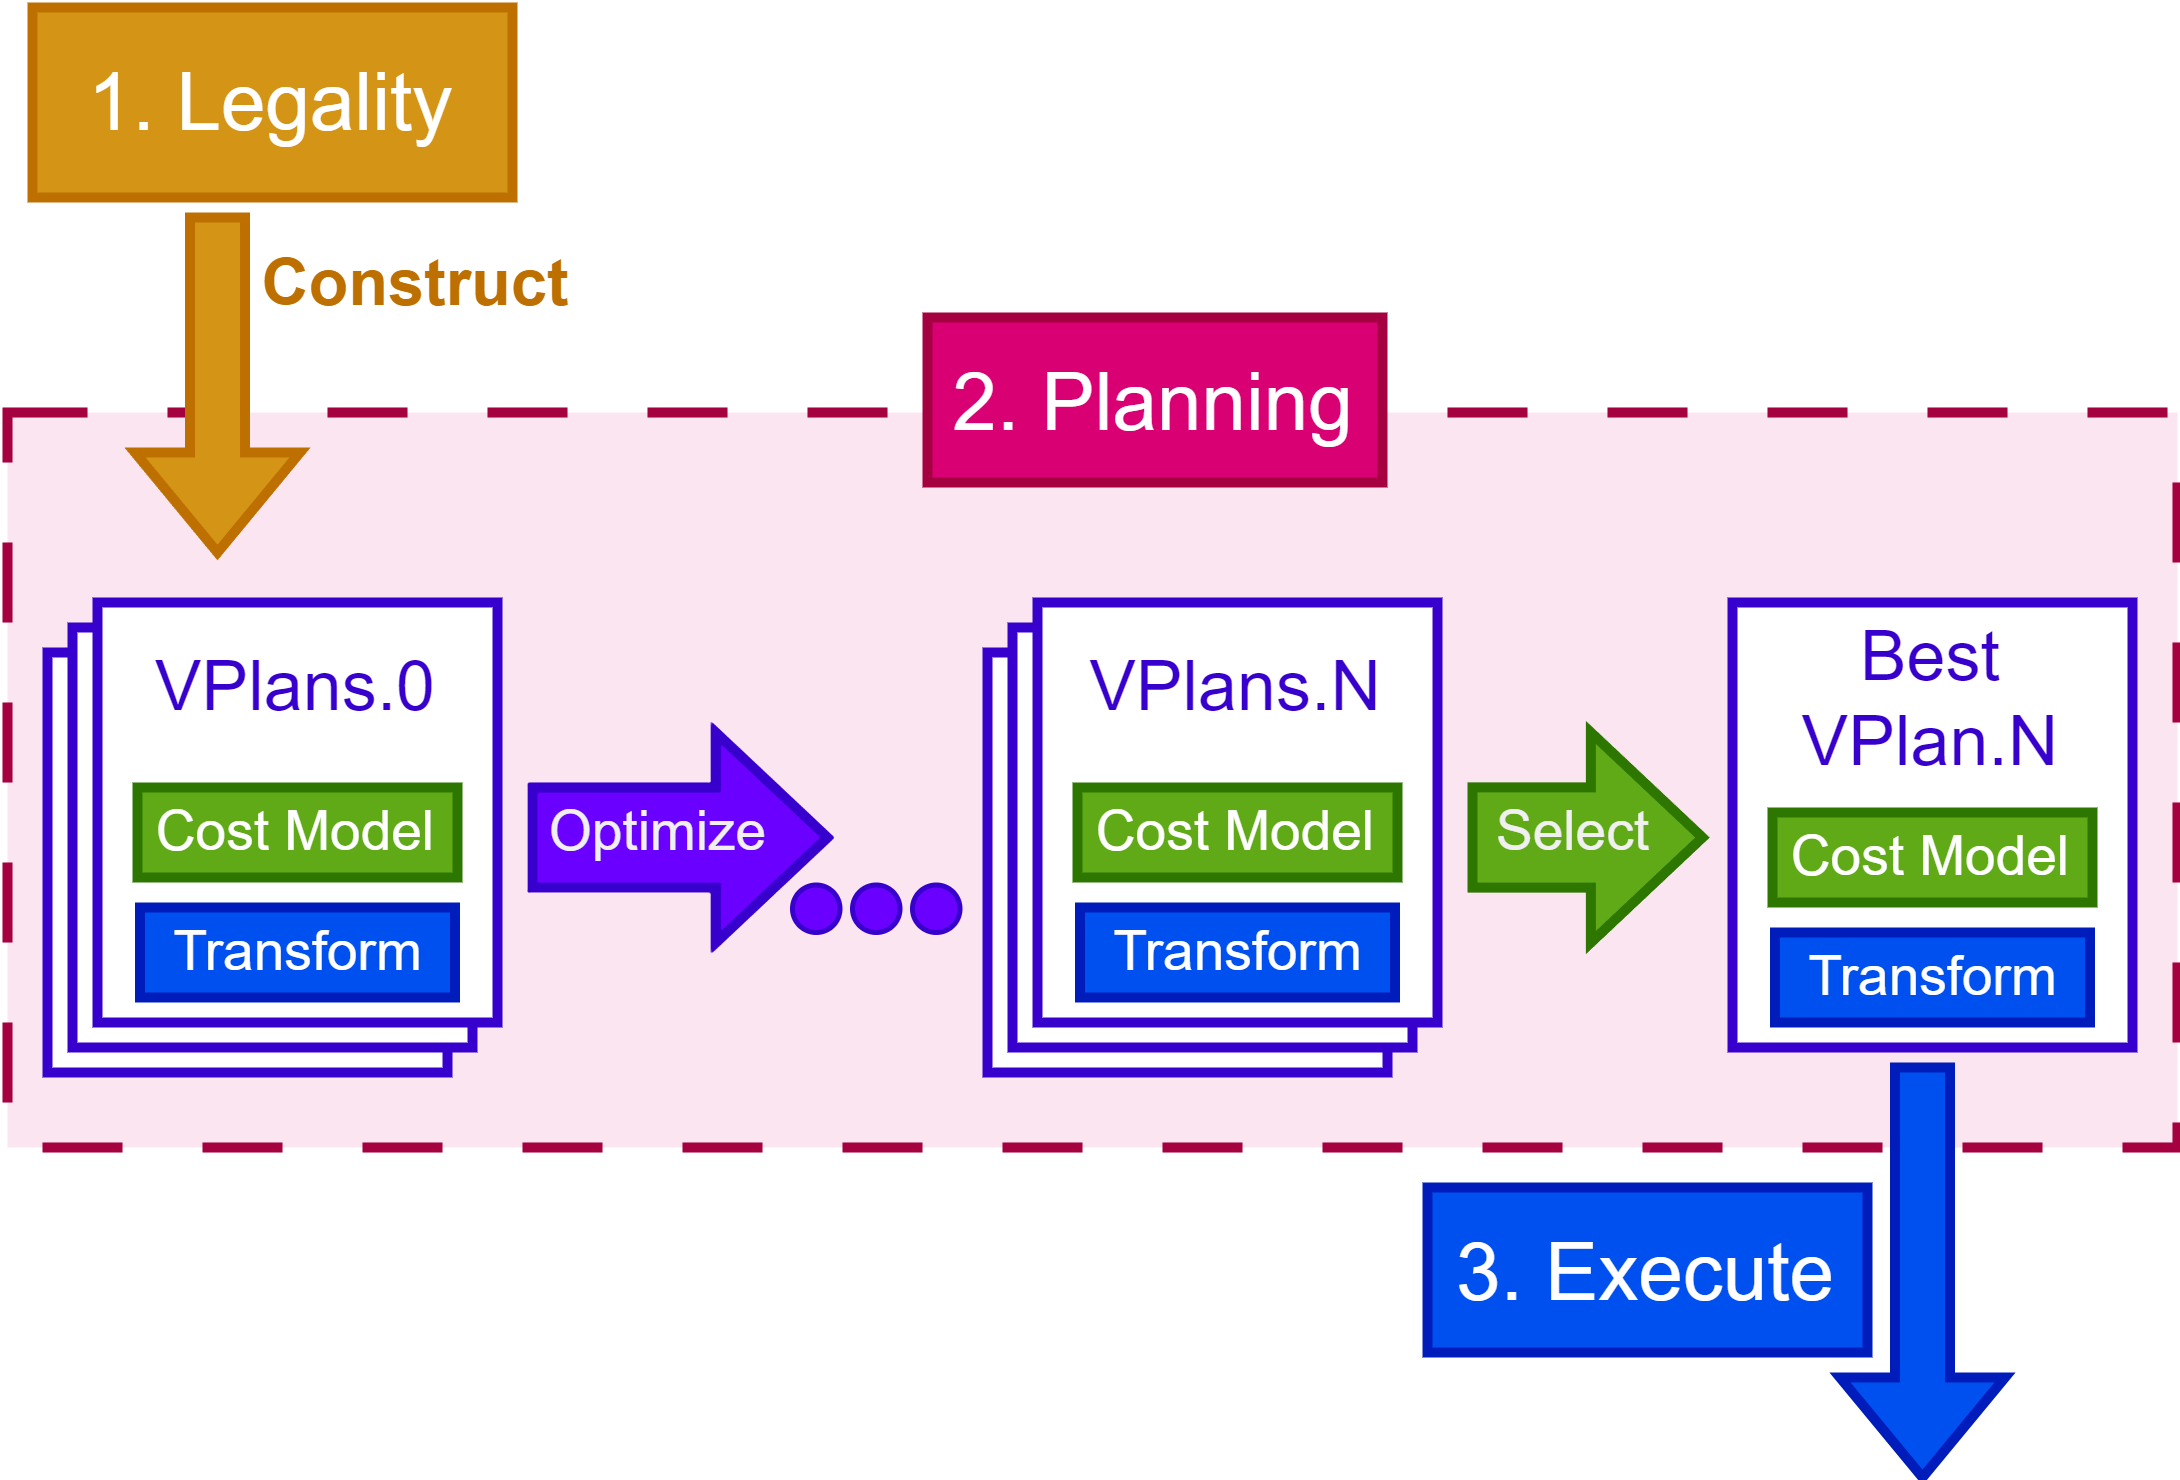
\includegraphics[width=0.475\textwidth]{images/vplan-future.png}
  \caption{The planned future architecture for auto-vectorization in LLVM. The 
  optimization step in phase 2 would iteratively apply VPlan-to-VPlan transformations.}
  \label{fig:vplan-future}
\end{figure}

\subsection{VPlan Structure}
Before explaining how far this system is already implemented in LLVM we will go over
the different elements of a \texttt{VPlan} in more detail.

The purpose of a single VPlan object is to model a candidate for vectorization. 
Such a single candidate can potentially represent multiple different vectorized loops in the end. 
For example, one VPlan might model a general vectorization approach for multiple different 
Vectorization Factors (VFs) and multiple different Unroll Factors (UFs) if applicable.

\paragraph{H-CFG}
This is achieved by introducing a new layer of abstraction from the underlying loop's scalar IR.
Each VPlan stores its own Hierarchical-CFG (H-CFG) modeling the vectorization candidate. This 
control-flow graph and its components are the main element of a single VPlan.
The nodes of this H-CFG are one of three types:

\begin{itemize}
  \item \texttt{VPBasicBlock} stores a list of \texttt{VPRecipes}, similar to 
  the LLVM IR's \texttt{BasicBlock} holding a list of IR Instructions.
  \item \texttt{VPRegionBlock} represents a subgraph with a single VP entry node and a 
  single VP exit node. A \texttt{VPRegionBlock} can be marked to replicate its subgraph
  \texttt{VF * UF} times when executing. This is useful for modeling scalarized or predicated
  instructions within the final vectorized loop body.
  \item \texttt{VPIRBasicBlock} is a special \texttt{VPBasicBlock} that wraps an underlying
  IR \texttt{BasicBlock}. These nodes are useful for modeling the scalar parts around the 
  final vectorized loops such as the loop preheader and the epilogue loop.
\end{itemize}

Figure~\ref{fig:inner-loop-scalar-ir} shows the loop part of the scalar IR for the code example
of Figure~\ref{fig:inner-loop-vec}. Comparatively, Figure~\ref{fig:inner-loop-vplan-hcfg-body}
shows the loop part of the H-CFG of a VPlan that models the vectorization approach described
in Figure~\ref{fig:inner-loop-vec}.

\begin{figure}
  \centering
  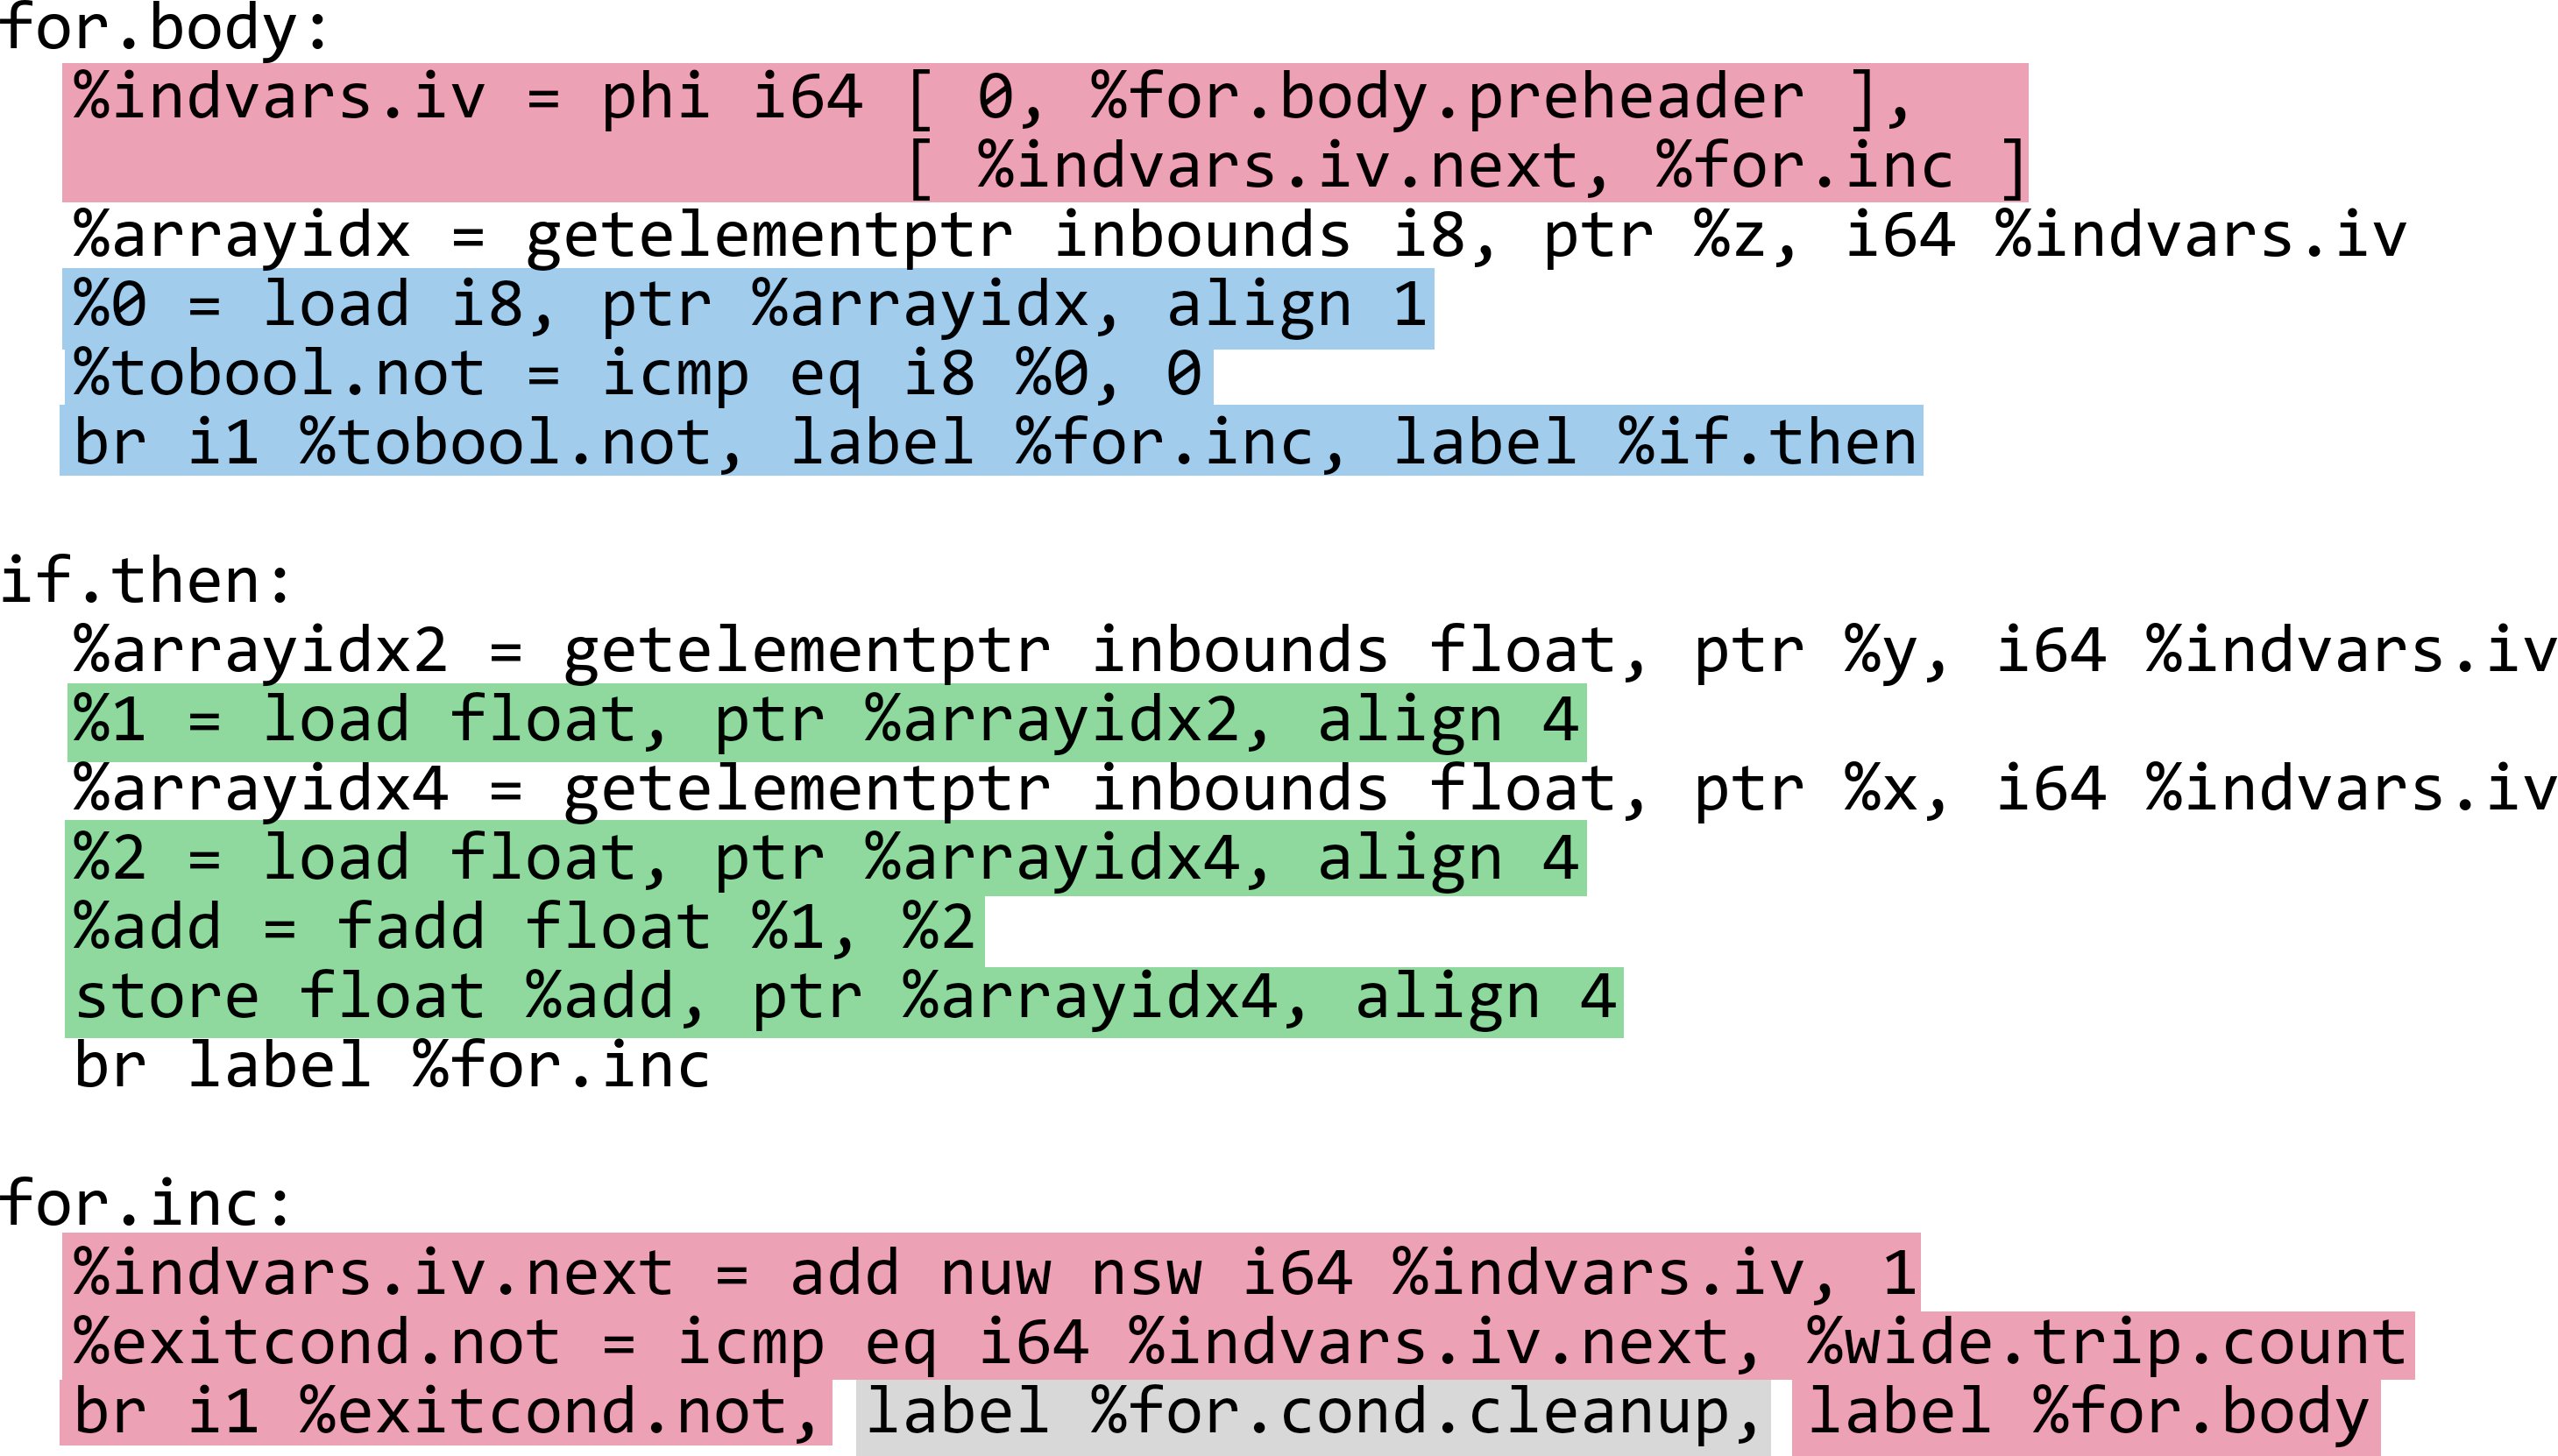
\includegraphics[width=0.475\textwidth]{images/inner-loop-scalar-loop-ir-color.png}
  \caption{The scalar IR for the main loop section of the conditional loop depicted in
  Figure~\ref{fig:inner-loop-vec}. Note that \texttt{getelementptr inbounds}
  was abbreviated to \texttt{getelmptr inbs}.}
  \label{fig:inner-loop-scalar-ir}
\end{figure}

\begin{figure}
  \centering
  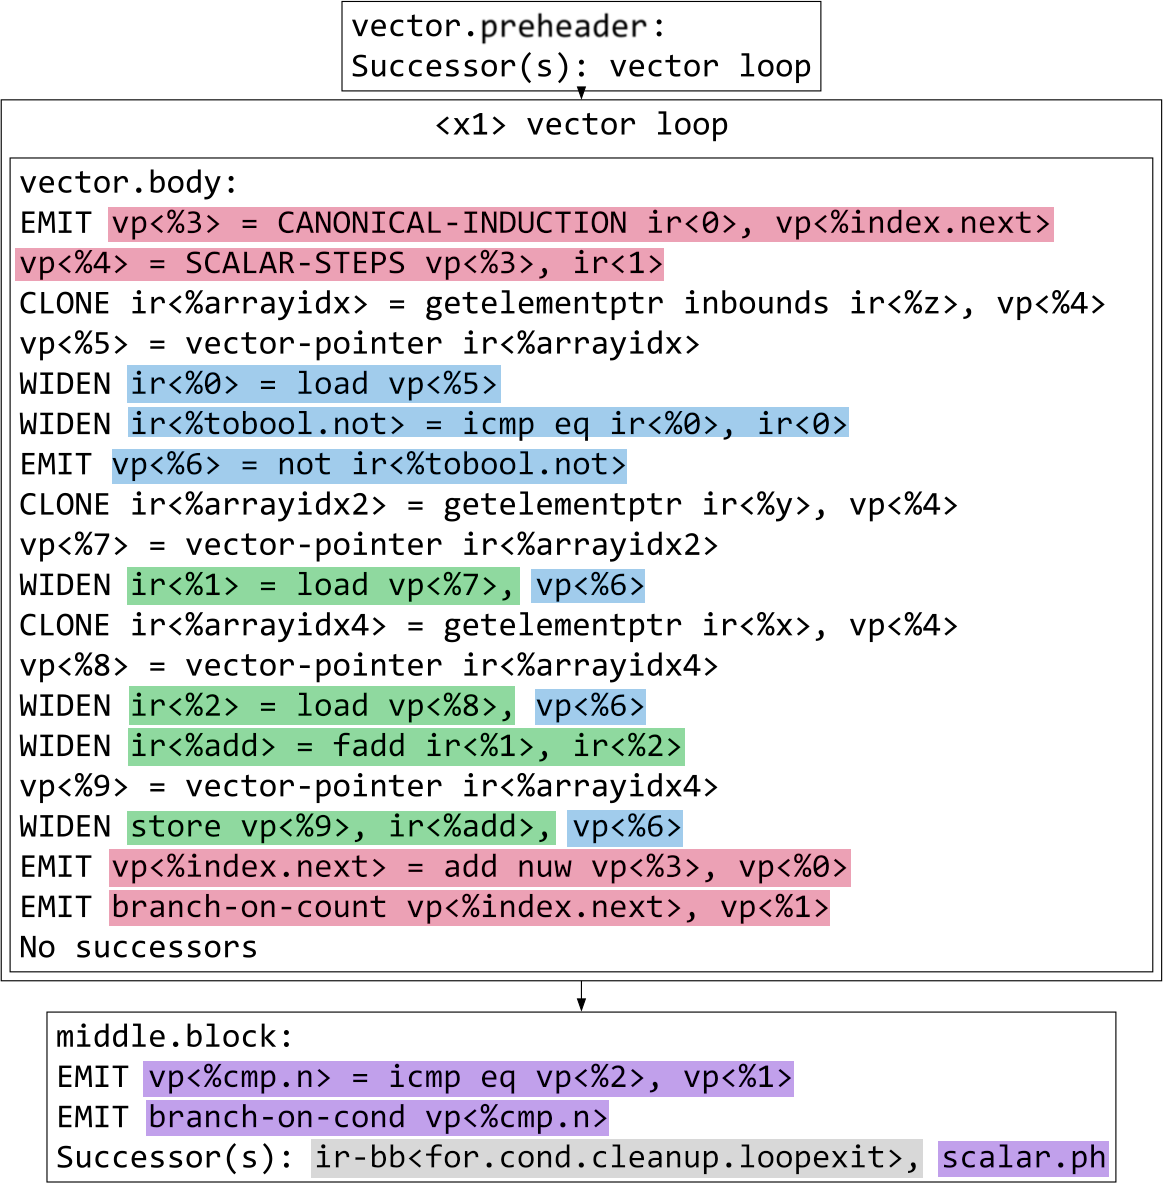
\includegraphics[width=0.475\textwidth]{images/inner-loop-vplan-hcfg-loop-body-color.png}
  \caption{The vectorized loop section of the hierarchical CFG of a VPlan modeling the 
  conditional loop depicted in Figure~\ref{fig:inner-loop-vec}. 
  Surrounding \texttt{VPIRBasicBlock}-nodes are omitted.
  Some predefined values are
  \texttt{vp<\%0>} = VF * UF; \texttt{vp<\%1>} = vector-trip-count; \texttt{vp<\%2>} = original trip-count.}
  \label{fig:inner-loop-vplan-hcfg-body}
\end{figure}

\paragraph{Recipes}

\texttt{VPRecipes} can be seen as instructions of an IR specialized for auto-vectorization. 
A single \texttt{VPRecipe} inside a VPlan is based on zero or more LLVM IR instructions of the 
underlying scalar IR and will materialize into one or more LLVM IR instructions when executed.

There are many different types of \texttt{VPRecipes}, most notably:
\begin{itemize}
  \item \texttt{VPReplicateRecipe} will replicate one IR instruction either once (\texttt{CLONE})
  or multiple times (\texttt{REPLICATE}) into the vectorized IR when executed.
  \item \texttt{VPWidenRecipe} will \texttt{WIDEN} one IR instruction into a
  vector-equivalent when executed.
  \item \texttt{VPInstruction} has no underlying IR instruction it is based on and is used 
  to model newly needed instructions for the vectorized IR. When executed it will 
  \texttt{EMIT} one or more new IR instructions.
\end{itemize}

The \texttt{VPRecipes} in Figure~\ref{fig:inner-loop-vplan-hcfg-body} have a \texttt{PREFIX}
infront of them indicating their type. Additionally instructions/recipes of the same color 
between Figure~\ref{fig:inner-loop-scalar-ir} and Figure~\ref{fig:inner-loop-vplan-hcfg-body}
are related. The only recipes in our example VPlan CFG that do not semantically model any 
instructions found in the scalar IR are from the \texttt{middle.block} (purple). This block 
is used to decide if the scalar epilogue loop is to be executed following the vectorized loop.

\paragraph{Transformations}
Another main benefit of the modular VPlan system is that most vector-optimization cases can 
be directly implemented as standalone VPlan-to-VPlan transformations. A VPlan-to-VPlan 
transformation is a static method that either transforms a given VPlan or creates a new 
VPlan based on a given VPlan. The analysis for these transformations can also be done 
directly on the VPlan via its \texttt{VPRecipes}.

\subsection{State of VPlan (LLVM 19.1.4)}
\emergencystretch 6em
In its current state, VPlan is already deeply integrated into LoopVectorize (LV) and is
used to model, optimize and execute vectorization of innermost loops~\cite{llvmvplan,llvmintrvplan,llvmvplanupdate}. 
While outer loop vectorization via VPlan has already seen quite some development, any 
outer loop vectorization features are still experimental and need to be explicitly enabled 
by passing the \texttt{-enable-\allowbreak vplan-\allowbreak native-\allowbreak path} 
feature flag~\cite{llvmouterloop,llvmouterloopstatus}.

To better understand how VPlan is already being used in LLVM, we will now follow along the 
LoopVectorize pass and summarize its key components.

\subsubsection{Phase 1: Legality}
The main part of this phase is checking whether it is even legal to optimize a given loop. 
In addition to the general vectorization legality concepts mentioned in 
Section~\ref{sec:vec-legal}, LV has a number of extra conditions to check.

Some of the most important legality checks done are:
\begin{itemize}
  \item The scalar loop's control flow must not contain indirect branches or multiple backedges.
  An indirect branch is a branch that jumps to a value evaluated at runtime. A backedge in a loop 
  is an edge from the loop back to it. 
  \item Loops with non-linear control flow must be if-convertible. This means any branch or switch 
  statement must not exit the loop, all instructions of such a block can be executed speculatively 
  (e.g. via masking)
  \item Loop-carried dependencies must be vectorizable (see Section~\ref{sec:vec-legal}). In LV 
  this means explicitly that such a value must \textit{at least} either be an induction variable, a reduction 
  variable, or a fixed-order recurrence.
  \item The loop must not contain function calls outside of standard math library calls.
  \item Types must be vectorizable. Vectorizable types are integers, floating point types, and 
  pointers.
  \item The number of runtime checks to guarantee no pointers used by recurrences overlap must not be too high.
\end{itemize}

One can find a lot more details about these legality checks and their implementations by looking 
at the LLVM codebase under \texttt{LoopVectorizationLegality::\allowbreak canVectorize}.

\subsubsection{Phase 2: Planning}
After the Legality Phase has analyzed the scalar loop, initial VPlans are constructed.
A VPlan is initialized by first creating the H-CFG skeleton building blocks like preheaders, a 
region block for the vector loop, a middle block with the potential runtime check for the scalar 
epilogue loop, and a block for the scalar loop. After the H-CFG has been created, the scalar LLVM IR 
is iterated in topological order and each scalar IR instruction is transformed into a \texttt{VPRecipe}.
After finishing modeling each scalar IR instruction into the VPlan, a number of VPlan transformations 
are executed, optimizing the initialized VPlan.

After the initial VPlans have been optimized the best Vectorization Factor is computed. This is done 
by comparing all generated VPlans for all their possible VFs and choosing the most profitable one. If 
this step computes a optimal VF of $1$, it means that any form of vectorization is not profitable.

\paragraph{Cost Model}
Currently LV and VPlan still mostly rely on the old cost model. This legacy cost model derives costs 
based on the scalar LLVM IR instructions or, if applicable, their vectorized equivalent.
This is suboptimal for VPlan as VPlans work on \texttt{VPRecipes} abstracted away from the underlying 
IR. These costs per instructions are then generally just lookup tables influenced by the underlying 
compile target. 

\subsubsection{Phase 3: Execution}
After the best VPlan has been chosen it is executed (\texttt{LoopVectorizationPlanner::executePlan}).
For this VPlan some final transformations are made that depend on a specifically chosen VF and UF.
First a vectorized code skeleton is created in the IR, then the VPlan is executed. Upon execution 
the H-CFG of the VPlan is walked and each node is executed, which in turn executes all of its 
\texttt{VPRecipes} in order.

Figure~\ref{fig:inner-loop-vec-cfg} shows the general CFG of a vectorized loop in LLVM and for branches 
the general branch condition per block.

\begin{figure}
  \centering
  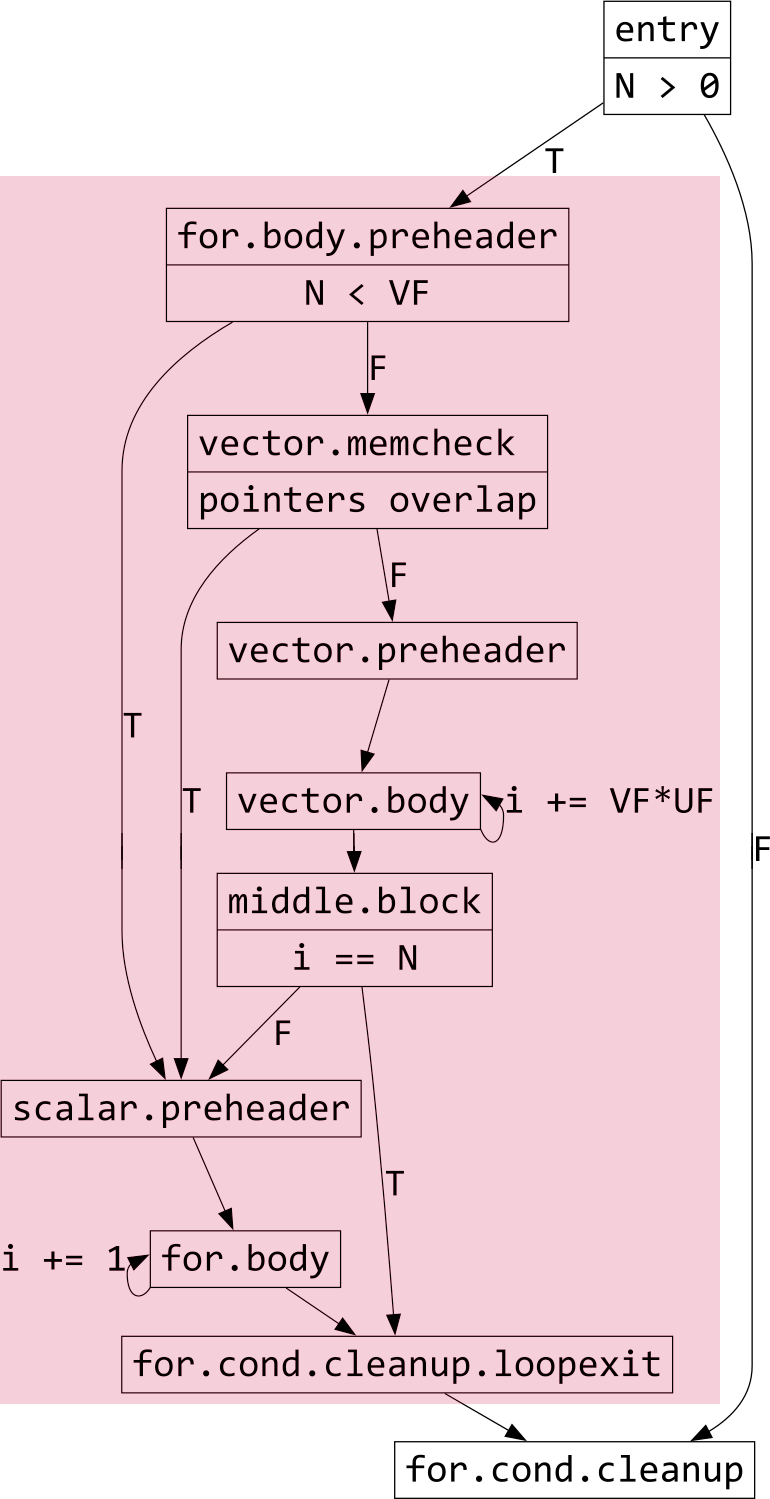
\includegraphics[width=0.35\textwidth]{images/inner-loop-vec-loop-cfg-color.png}
  \caption{The generalized CFG for a vectorized loop with trip count \texttt{N}, 
  iteration variable \texttt{i}, vectorization factor \texttt{VF}, 
  and unroll factor \texttt{UF} in LLVM. A VPlan would explicitly model the red-highlighted 
  region in its H-CFG.}
  \label{fig:inner-loop-vec-cfg}
\end{figure}

In case that the epilogue loop could also be further vectorized, it will be in a second 
pass by creating VPlans for it, finding the best one and executing it.

\subsection{Future of VPlan}
Many of the VPlan internals and surrounding systems are still in active development. To stay up-to-date 
with the latest developments regarding auto-vectorization in LLVM, one can follow the 
Community Forum\footnote{\url{https://discourse.llvm.org/c/ir-optimizations/loop-optimizations/62}} or
attend the monthly online 
meetings\footnote{\url{https://discourse.llvm.org/t/monthly-vectorizer-online-sync-up/78978/3}}.

\subsubsection{VPlan and Integration with LV}
Setting up and integrating the VPlan structure into LV has seen tremendous effort over the last 
few years. Florian Hahn presented future directions for 
VPlan~\cite{llvmvplanupdate}, which mostly revolve around transforming more LV-based decisions into
explicit VPlan-to-VPlan transformations. Additionally, the legacy LV cost model still influences 
many cost model-related decisions. However, the transition to a VPlan-based cost model has already 
started. This new model would derive costs based on \texttt{VPRecipes} directly instead of the 
abstracted scalar IR instructions.

\subsubsection{Outer Loop Vectorization}
Development around outer loop vectorization has slowed as the focus shifted to VPlan internals 
and integration into LV. The inner and outer loop paths are still separated, and the 
experimental \texttt{-enable-\allowbreak vplan-\allowbreak native-\allowbreak path} flag must be 
set to activate any outer 
loop vectorization. Further development of the outer loop path and eventually merging it 
with the innermost loop path is planned.

\subsubsection{Merging with SLP Vectorize}
Merging the existing SLP Vectorizer with the current VPlan infrastructure is in the early planning phase.

\subsubsection{Function Vectorization}
There is currently no active development for whole-function vectorization in the
llvm-project's upstream.


%%%%%%%%%%%%%%%%%%%%%%%%%%%%%%%%%%%%%%%%%%%%%%%%%%%%%%%%%%%%%%%%%%%%%%%%%%%%%%%%%%%%%%%%%%%%%%%%%%%%%%
%%%%%%%%%%%%%%%%%%%%%%%%%%%%%%%%%%%%%%%%%%%%%%%%%%%%%%%%%%%%%%%%%%%%%%%%%%%%%%%%%%%%%%%%%%%%%%%%%%%%%%
%%%%%%%%%%%%%%%%%%%%%%%%%%%%%%%%%%%%%%%%%%%%%%%%%%%%%%%%%%%%%%%%%%%%%%%%%%%%%%%%%%%%%%%%%%%%%%%%%%%%%%


\section{Related Work}
\label{sec:relatedwork}
Next to the main llvm-projects upstream, many projects are using or extending the LLVM toolchain.

One such project that tries to enable auto-vectorization support for inner/outer loops and 
whole-functions is the region vectorizer (RV) from the University Saarland~\cite{rv}.
The idea is that all the different vectorization strategies shown in Section~\ref{back:vec-strat}
can be generalized into a single vectorization approach.

For example, function vectorization can be transformed into loop vectorization by creating a loop 
around the function's body and vectorizing it and vice versa. 
The same applies for SLP Vectorization and loop vectorization by unrolling a loop.

RV's goal is to have such a generalized auto-vectorization by vectorizing over \textit{regions}.
A region is defined as any control flow that has a single entry and one or more non-divergent exits.
Non-divergent exits mean that starting from the same entry, control flow must not diverge to different
exits.
Such a region can then be for example an inner/outer loop, function, or SLP code~\cite{rvintro,rvproposal}.

To achieve this, RV implements partial control-flow linearization~\cite{10.1145/3192366.3192413}
and a divergence analysis that can handle unstructured CFGs. There has been an effort to partially
implement this control-flow linearization and divergence analysis into LLVM's 
upstream~\cite{rvproposal,rvproposaldep}.

%%%%%%%%%%%%%%%%%%%%%%%%%%%%%%%%%%%%%%%%%%%%%%%%%%%%%%%%%%%%%%%%%%%%%%%%%%%%%%%%%%%%%%%%%%%%%%%%%%%%%%
%%%%%%%%%%%%%%%%%%%%%%%%%%%%%%%%%%%%%%%%%%%%%%%%%%%%%%%%%%%%%%%%%%%%%%%%%%%%%%%%%%%%%%%%%%%%%%%%%%%%%%
%%%%%%%%%%%%%%%%%%%%%%%%%%%%%%%%%%%%%%%%%%%%%%%%%%%%%%%%%%%%%%%%%%%%%%%%%%%%%%%%%%%%%%%%%%%%%%%%%%%%%%


\section{Summary and Future Work}
\label{sec:summary}
In conclusion, VPlan has been in active development for several years now. When compiling with LLVM, 
VPlans are used to model different vectorization approaches. They do so by adding a new layer of 
abstraction over the underlying LLVM IR. This VPlan layer uses \texttt{VPRecipes} to model vectorization 
specific instructions. This abstraction allows for efficiently exploring many different optimization 
decisions at once, keeping the underlying implementation flexible and modular. In the end a cost model, 
currently still working based on LLVM IR instead of \texttt{VPRecipes} is used to compare different VPlans 
and choose the most optimal one. Finally this chosen VPlan is executed, materializing its \texttt{VPRecipes} 
back into LLVM IR.

Outer loop vectorization support via VPlan is still experimental and separated from the inner loop
LV integration. In the near future, development on outer loop vectorization will continue, and merging 
it with LV's VPlan path is planned.

Active development of other approaches, such as SLP and whole-function vectorization based on the VPlan 
architecture, has yet to be started.

%%%%%%%%%%%%%%%%%%%%%%%%%%%%%%%%%%%%%%%%%%%%%%%%%%%%%%%%%%%%%%%%%%%%%%%%%%%%%%%%%%%%%%%%%%%%%%%%%%%%%%
%%%%%%%%%%%%%%%%%%%%%%%%%%%%%%%%%%%%%%%%%%%%%%%%%%%%%%%%%%%%%%%%%%%%%%%%%%%%%%%%%%%%%%%%%%%%%%%%%%%%%%
%%%%%%%%%%%%%%%%%%%%%%%%%%%%%%%%%%%%%%%%%%%%%%%%%%%%%%%%%%%%%%%%%%%%%%%%%%%%%%%%%%%%%%%%%%%%%%%%%%%%%%

\bibliographystyle{ACM-Reference-Format}
\bibliography{paper} % read paper.bib file

\end{document}
